\chapter{Structural view}

\section{Introduction}
This chapter describes the structural architecture of the system in a top down approach.\\
The blocks are derived from previous documentation.


\section{System overview}
The system consist of a central data unit and n number of sensors.
\begin{figure}[hbpt]
\centering
\includegraphics[width=.9\textwidth]{billeder/systembdd}
\caption{System block definition diagram}
\label{systembdd}
\end{figure}

\subsection{Block responsibility}
\subsubsection{CDU}
The CDU contacts each sensor to collect the data values. This is then stored for later extraction.

\subsubsection{Sensor node n}
The sensor node measures a physical or biometric parameter such as temperature, movement, humidity etc.

\section{Detailed block overview}
Below are detailed figures for each block in the system.\\
The blocks in the figures are conceptual blocks and most of the consist of both software and hardware.\\
All blocks are essential to fulfil the functionality and requirements of the system.

\subsection{CDU}

\begin{figure}[hbpt]
\centering
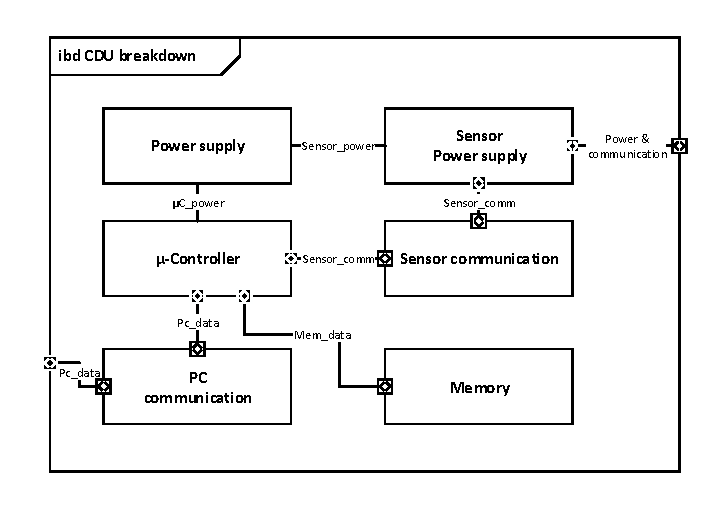
\includegraphics[width=.8\textwidth]{billeder/CDU_IBD}
\caption{Internal Block Diagram of the CDU}
\label{CDU_IBD}
\end{figure}

\subsubsection{Block description}

\textbf{Powersupply:}\\
The powersupply feeds the necessary power to the modules on which it is connected.\\
The voltage and current levels will be specified in the physical view.\\

\textbf{Sensor powersupply:}\\
The Sensor powersupply feeds the power needed to operate all sensors connected to the system.\\
The voltage and/or current levels will be specified in the physical view.\\

\textbf{µ-Controller:}\\
The µ-Controller runs the main application. Main objectives:\\
$\bullet$ Keep track of sensors\\
$\bullet$ Collect data\\
$\bullet$ Store data\\

\textbf{Sensor communication:}\\
The Sensor communication interfaces with the sensor powersupply to modulate the powerline to the sensor nodes.\\
The sensor communication block has no intelligence and the protocol is handled by the µ-Controller block.\\

\textbf{Memory:}\\
The memory stores all data collected by the µ-Controller. The memory can be detachable or some kind of eeprom/flash.\\

\textbf{PC communication:}\\
The PC communication is an interface to a PC. This can be USB, serial or any third option.\\


\subsection{Sensor node n}

\begin{figure}[hbpt]
\centering
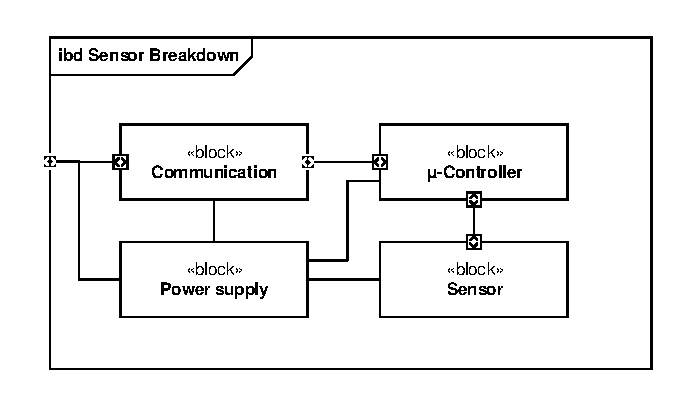
\includegraphics[width=.8\textwidth]{billeder/Sensor_IBD}
\caption{Internal Block Diagram of the sensor}
\label{Sensor_IBD}
\end{figure}

\subsubsection{Block description}

\textbf{Powersupply:}\\
The powersupply located in the sensor regulates the voltage and current levels to fit the need of the individual blocks in the sensor.\\

\textbf{Communication:}\\
The communication block demodulates the communcation on the input line and feeds it to the sensor logic.\\

\textbf{Logic handler;}\\
The logic handler interprets the incomming communication and responds accordingly.\\
It also handles sensor measurements.\\

\textbf{Sensor:}\\
The sensor block is mostly a physical element in the sensor node. It feeds a voltage or similar to the logic handler.\\



